\documentclass[11pt,a4paper]{article}

\usepackage[utf8]{inputenc}
\usepackage[T1]{fontenc}
\usepackage[brazilian]{babel}
\usepackage{lmodern}
\usepackage{amsmath,amssymb}
\usepackage{graphicx}
\usepackage{booktabs}
\usepackage{float}
\usepackage[margin=2.3cm]{geometry}
\usepackage{caption}
\usepackage{icomma}

\captionsetup{font=small,labelfont=bf}
\setlength{\parskip}{4pt}

\newcommand{\Vbar}{\bar{V}}
\newcommand{\code}[1]{\texttt{#1}}

\title{Trabalho Prático 1: Robô de Limpeza e Cachorro\\[4pt]
\large Tópicos Especiais em Aprendizado por Reforço, COS767-2026/3}
\author{Claudionor Ferreira da Silva Junior}
\date{04/11/2026}

\begin{document}
\maketitle

% =====================================================================
\section{Introdução e convenções}

Este relatório apresenta as implementações da seção 4 do enunciado e as respostas às tarefas da seção 5, para $p = 0{,}2$, $k \in \{0, 1, 2, 4, 6, 10\}$ e $\gamma$ igual a $0{,}7$ ou $0{,}99$, na sala do enunciado (606.816 estados). Os métodos utilizados são avaliação de política, iteração por política, iteração por valor e Q-learning. O MDP de cada $k$ foi construído uma vez com \code{TabularModel} e guardado em disco, já que não depende de $\gamma$.

A recompensa é $r(s) = -1$ com xixi na sala e $0$ com a sala limpa. Dada uma política $\pi$, o MDP vira um MRP com matriz de transição
\[
P_\pi(s, s') = \sum_a \pi(a \mid s)\, p(s' \mid s, a),
\]
e o valor dos estados satisfaz $V^\pi = r + \gamma P_\pi V^\pi$. A política ótima é denotada por $\pi^\circ$.

\subsection*{Medida de desempenho}

Para resumir o valor dos estados em um número, usa-se a média de $V^\pi$ sobre a distribuição inicial $\nu(0)$ do ambiente, chamada aqui de $\Vbar$. O \code{random\_init} sorteia de forma uniforme os estados com o cachorro em modo normal, que correspondem à primeira metade dos índices, então $\Vbar$ é a média simples de $V^\pi$ nesses estados. Quanto mais perto de zero, melhor.

Como $r(s)$ está entre $-1$ e $0$, o pior valor possível é
\[
-(1 + \gamma + \gamma^2 + \dots) = -\frac{1}{1-\gamma},
\]
que corresponde à sala suja para sempre, e vale $-3{,}33$ para $\gamma = 0{,}7$ e $-100$ para $\gamma = 0{,}99$. Esse pior caso serve de referência, pois a escala de $\Vbar$ depende de $\gamma$.

Também se usa a perda $V^{\pi^\circ}(s) - V^\pi(s)$, que mede quanto uma política fica abaixo da ótima, e a fração de estados em que a ação da política não é a de maior $Q$. Como a política ótima não é única, diferenças de $Q$ menores que $10^{-6}$ contam como empate. Perda e ação não ótima são nomes adotados neste relatório.

\subsection*{Observação sobre o reinício do robô}

Conforme a especificação do MDP, as $k$ rodadas de uma captura formam uma única transição, com recompensa $r(s)$, o que preserva a propriedade de Markov. O próximo estado é a distribuição do cachorro após $k$ rodadas em modo normal, e a recompensa e o desconto são aplicados uma só vez. Assim, o efeito de $k$ sobre o valor vem do que acontece nessas rodadas, em que o robô fica parado enquanto o cachorro se afasta e pode fazer um novo xixi.

% =====================================================================
\section{Implementações (seção 4)}

\code{policy\_evaluation} monta $P_\pi$ pela fórmula acima e usa o método iterativo, que parte de $V_0 = 0$ e repete $V_k = r + \gamma P_\pi V_{k-1}$ até que a maior variação entre duas iterações fique abaixo de $10^{-10}$.

\code{ValueIteration} repete
\[
V_{k+1}(s) = \max_a \Big( r(s) + \gamma \sum_o p(o \mid s, a)\, V_k(o) \Big)
\]
com o mesmo critério de parada e, ao final, escolhe em cada estado a ação de maior valor. \code{PolicyIteration} parte de uma política sorteada e alterna avaliação e melhoria até que a política não mude. A ação só é trocada quando a melhora em $Q$ passa de $10^{-6}$, para que empates não façam a política oscilar.

\code{QLearning} segue o algoritmo para ambiente sem estado terminal, com $Q = 0$, estado inicial sorteado, uma única trajetória, política $\varepsilon$-gulosa com $\varepsilon = 0{,}1$ e taxa de aprendizado $\alpha_m = 1/m$, em que $m$ é o número de visitas ao par $(s, a)$. O modelo só é usado depois do treino, para avaliar a política aprendida.

% =====================================================================
\section{Item 1: políticas gulosa e aleatória}

A política gulosa (fornecida) anda até o xixi pelo menor caminho e ignora o cachorro, enquanto a aleatória escolhe cada ação com probabilidade $0{,}2$. A Figura~\ref{fig:v_item1} mostra $\Vbar$ das duas.

\begin{figure}[H]
\centering
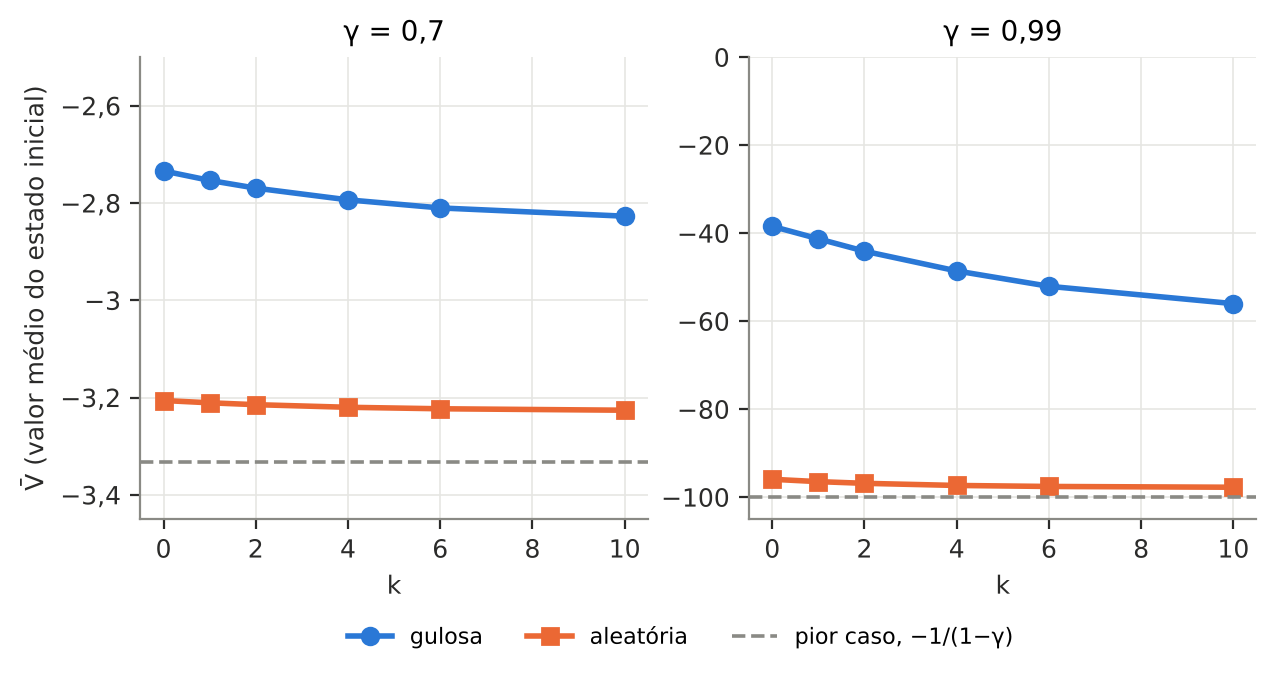
\includegraphics[width=0.85\textwidth]{fig/f1.png}
\caption{$\Vbar$ das políticas gulosa e aleatória em função de $k$. A linha tracejada é o pior caso.}
\label{fig:v_item1}
\end{figure}

\subsection*{1a. Quanto uma política perde em relação à outra}

A perda foi medida pela diferença de valores entre as duas políticas, estado a estado, $V^{\text{gulosa}}(s) - V^{\text{aleatória}}(s)$, e resumida pela média sobre os estados iniciais (Figura~\ref{fig:diferenca}). A gulosa é melhor em praticamente todos os estados, e a diferença média cai de $0{,}47$ para $0{,}40$ com $\gamma = 0{,}7$ e de 57 para 42 com $\gamma = 0{,}99$ quando $k$ vai de 0 a 10. A aleatória fica quase no pior caso (cerca de $-3{,}2$ e $-97$, Figura~\ref{fig:v_item1}), enquanto a gulosa fica bem longe dele com $\gamma = 0{,}99$.

\begin{figure}[H]
\centering
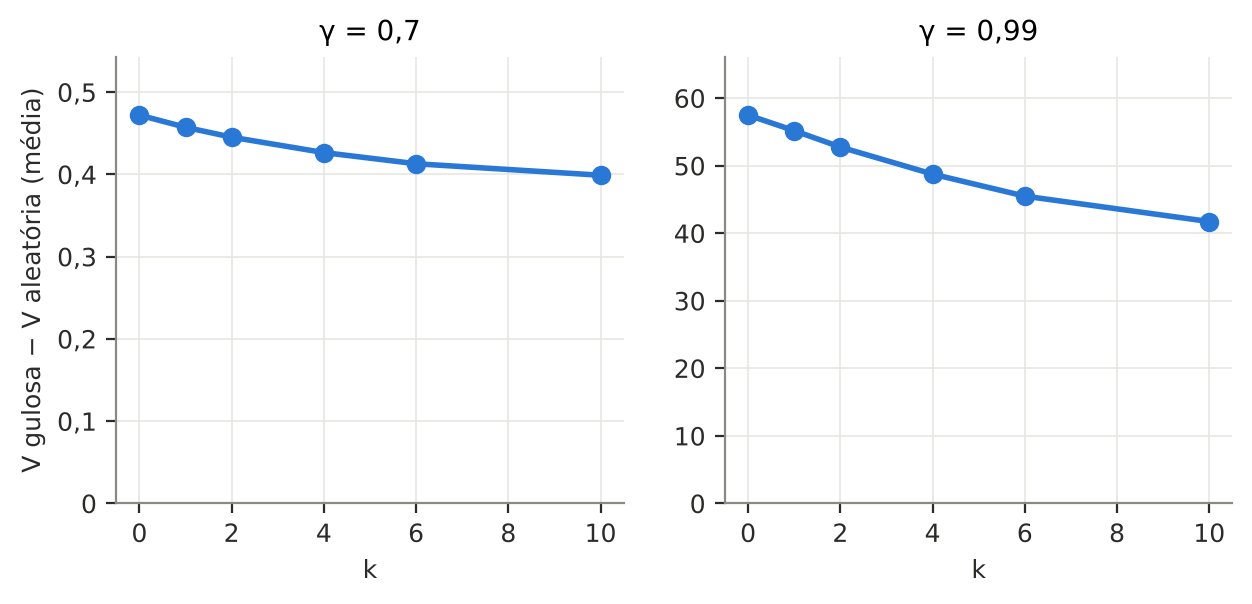
\includegraphics[width=0.85\textwidth]{fig/f9.png}
\caption{Diferença média de valor entre as políticas gulosa e aleatória em função de $k$. As escalas dos painéis são diferentes.}
\label{fig:diferenca}
\end{figure}

Uma trajetória simulada de 20.000 passos ajuda a interpretar esses valores. Pelo Teorema Ergódico, a média $S_k$ das recompensas ao longo da trajetória converge para a média de $r$ sob a distribuição estacionária, e como $r$ vale $-1$ ou $0$, $-S_k$ é a fração do tempo com a sala suja (Figura~\ref{fig:simulacao}). Com a gulosa essa fração vai de 35\% a 56\%, enquanto com a aleatória fica perto de 97\%.

\begin{figure}[H]
\centering
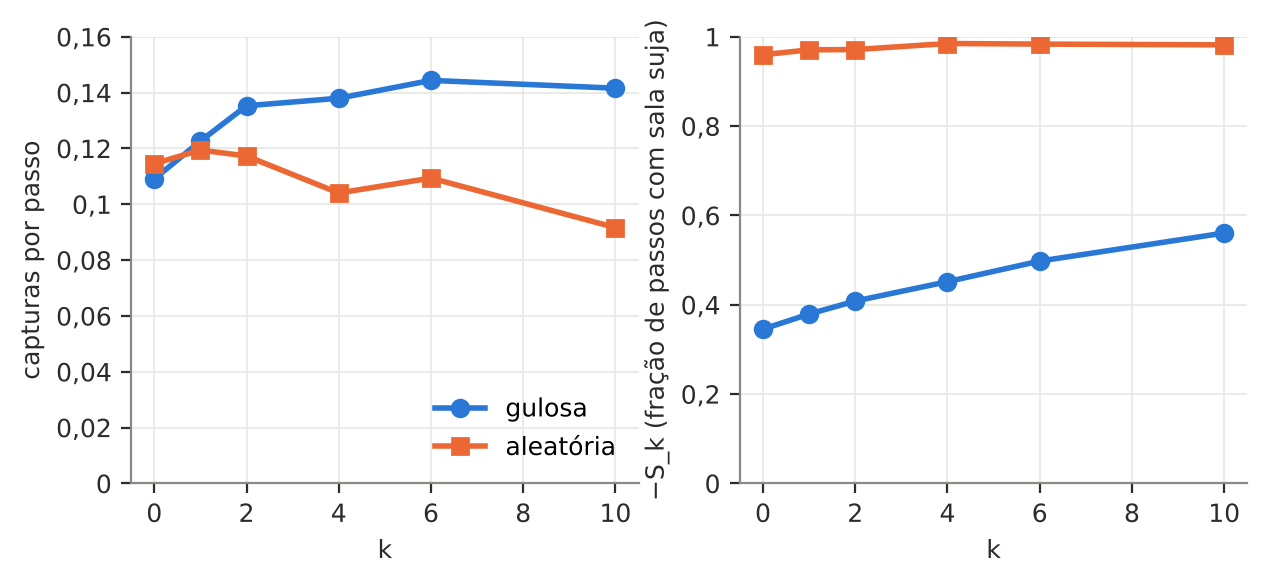
\includegraphics[width=0.85\textwidth]{fig/f2.png}
\caption{Trajetória simulada de 20.000 passos, com as capturas por passo e a fração do tempo com a sala suja.}
\label{fig:simulacao}
\end{figure}

\subsection*{1b. Variação com $k$ e com $\gamma$}

As duas políticas pioram com $k$. A gulosa é mais afetada porque ignora o cachorro, então é capturada mais vezes (de $0{,}11$ para cerca de $0{,}14$ por passo) e cada captura custa mais. A aleatória quase não muda porque já está perto do pior caso.

O fator de desconto define quanto o futuro pesa. Com $\gamma = 0{,}7$ só os primeiros passos importam, e como quase todo estado inicial começa com a sala suja, nenhuma política consegue mudar muito o valor, e por isso as curvas ficam próximas do pior caso e quase planas. Com $\gamma = 0{,}99$ importam cerca de 100 passos, e passa a contar quanto tempo a sala fica limpa entre um xixi e o seguinte. Por isso as diferenças entre políticas e o efeito de $k$ aparecem bem mais com $\gamma = 0{,}99$.

\subsection*{1c. Abordagem direta ou iterativa}

O método direto resolve o sistema $(I - \gamma P_\pi) V = r$, com custo $O(n^3)$, o que é inviável com $n = 606.816$ se a matriz for tratada como densa. Como $P_\pi$ é esparsa, os dois métodos foram comparados aproveitando isso, o direto com um resolvedor de sistemas esparsos do scipy e o iterativo com a repetição da equação. A comparação usou a política gulosa com $\gamma = 0{,}99$, o caso mais lento para o iterativo (Tabela~\ref{tab:1c} e Figura~\ref{fig:1c}).

\begin{table}[H]
\centering
\small
\begin{tabular}{rrrrrrr}
\toprule
estados & $k$ & iterações & \multicolumn{2}{c}{tempo (s)} & \multicolumn{2}{c}{memória (MB)} \\
\cmidrule(lr){4-5} \cmidrule(lr){6-7}
 & & & iterativo & direto & iterativo & direto \\
\midrule
23.520  & 2 & 2185 & 0,3  & 0,1  & 1  & 5   \\
67.200  & 2 & 2191 & 0,7  & 0,3  & 4  & 20  \\
115.200 & 2 & 2198 & 1,1  & 0,6  & 6  & 41  \\
296.208 & 2 & 2200 & 3,5  & 2,4  & 15 & 123 \\
\midrule
606.816 & 0 & 2186 & 6,3  & 7,9  & 16 & 230 \\
606.816 & 2 & 2203 & 10,4 & 11,8 & 29 & 325 \\
\bottomrule
\end{tabular}
\caption{Métodos iterativo e direto para a política gulosa com $\gamma = 0{,}99$. As quatro primeiras linhas são salas menores, e as duas últimas são a sala do enunciado. Os dois métodos deram o mesmo resultado.}
\label{tab:1c}
\end{table}

\begin{figure}[H]
\centering
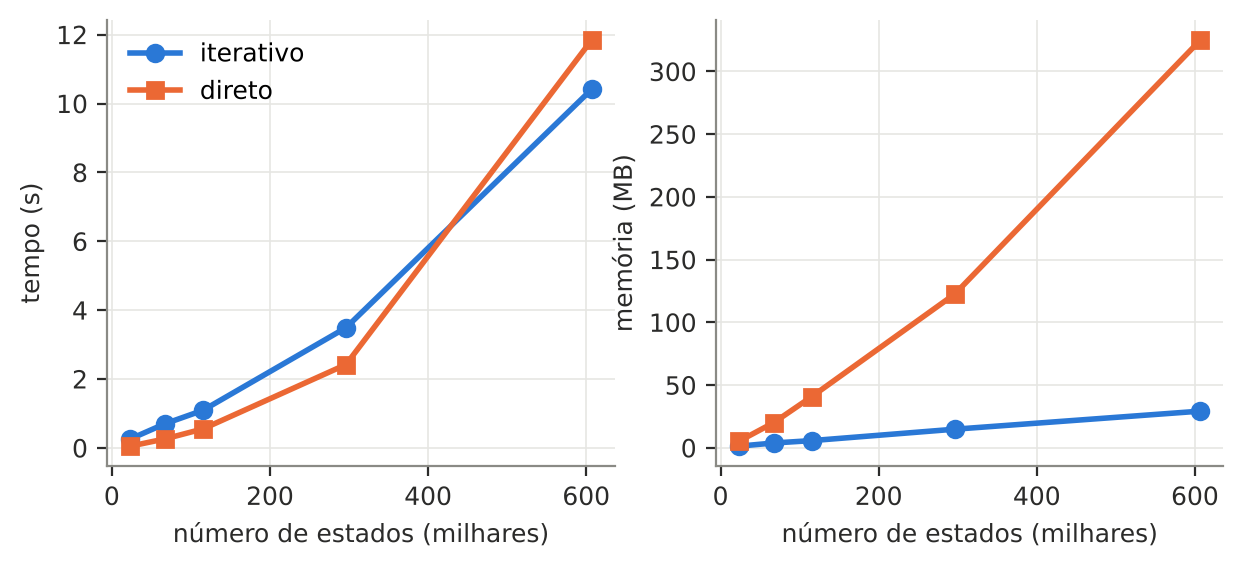
\includegraphics[width=0.8\textwidth]{fig/f3.png}
\caption{Tempo e memória dos dois métodos em função do número de estados ($k = 2$).}
\label{fig:1c}
\end{figure}

Nas salas pequenas o direto foi mais rápido, mas na sala do enunciado o iterativo já levou menos tempo. A diferença principal está na memória, já que o iterativo só guarda $P_\pi$ e dois vetores, enquanto o direto usou de 11 a 15 vezes mais memória, e essa diferença cresce com o tamanho do problema. Além disso, o sistema precisaria ser resolvido de novo a cada política avaliada. Por isso o método iterativo é o mais apropriado aqui, e seu ponto fraco é o número de iterações, cerca de 2200 com $\gamma = 0{,}99$ contra cerca de 60 com $\gamma = 0{,}7$.

% =====================================================================
\section{Item 2: iteração por política e iteração por valor}

Os dois métodos chegaram ao mesmo valor ótimo em todos os cenários. As Figuras~\ref{fig:tempo} e~\ref{fig:iteracoes} mostram tempo e iterações, e os tempos não incluem a construção do modelo.

\begin{figure}[H]
\centering
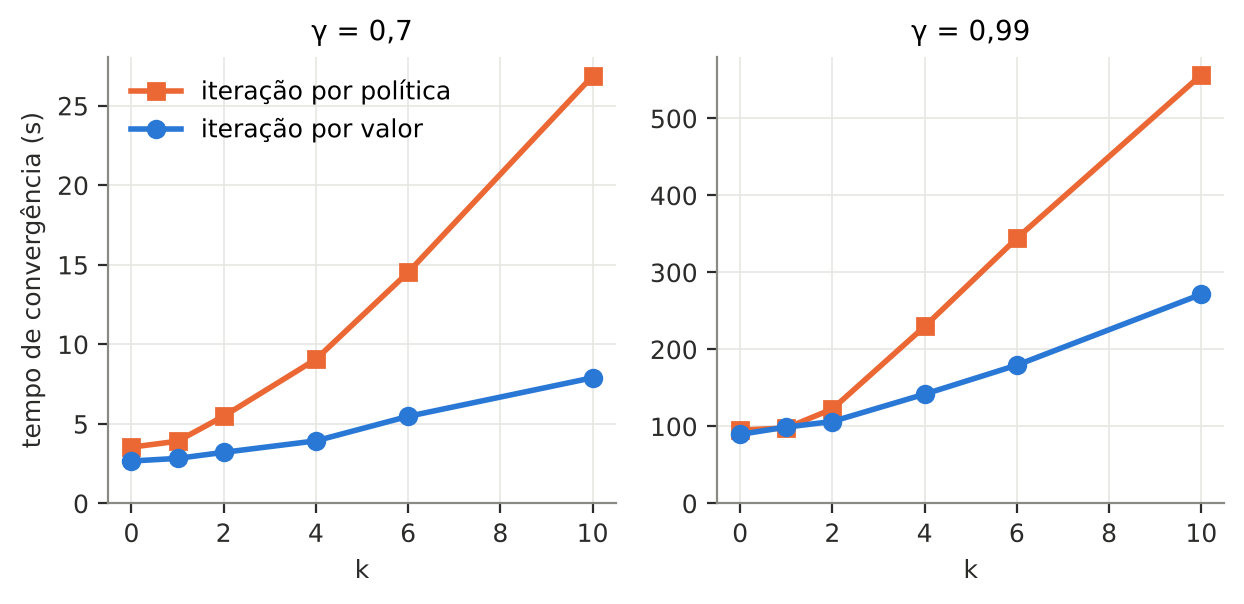
\includegraphics[width=0.85\textwidth]{fig/f4.png}
\caption{Tempo de convergência em função de $k$. As escalas dos painéis são diferentes.}
\label{fig:tempo}
\end{figure}

\begin{figure}[H]
\centering
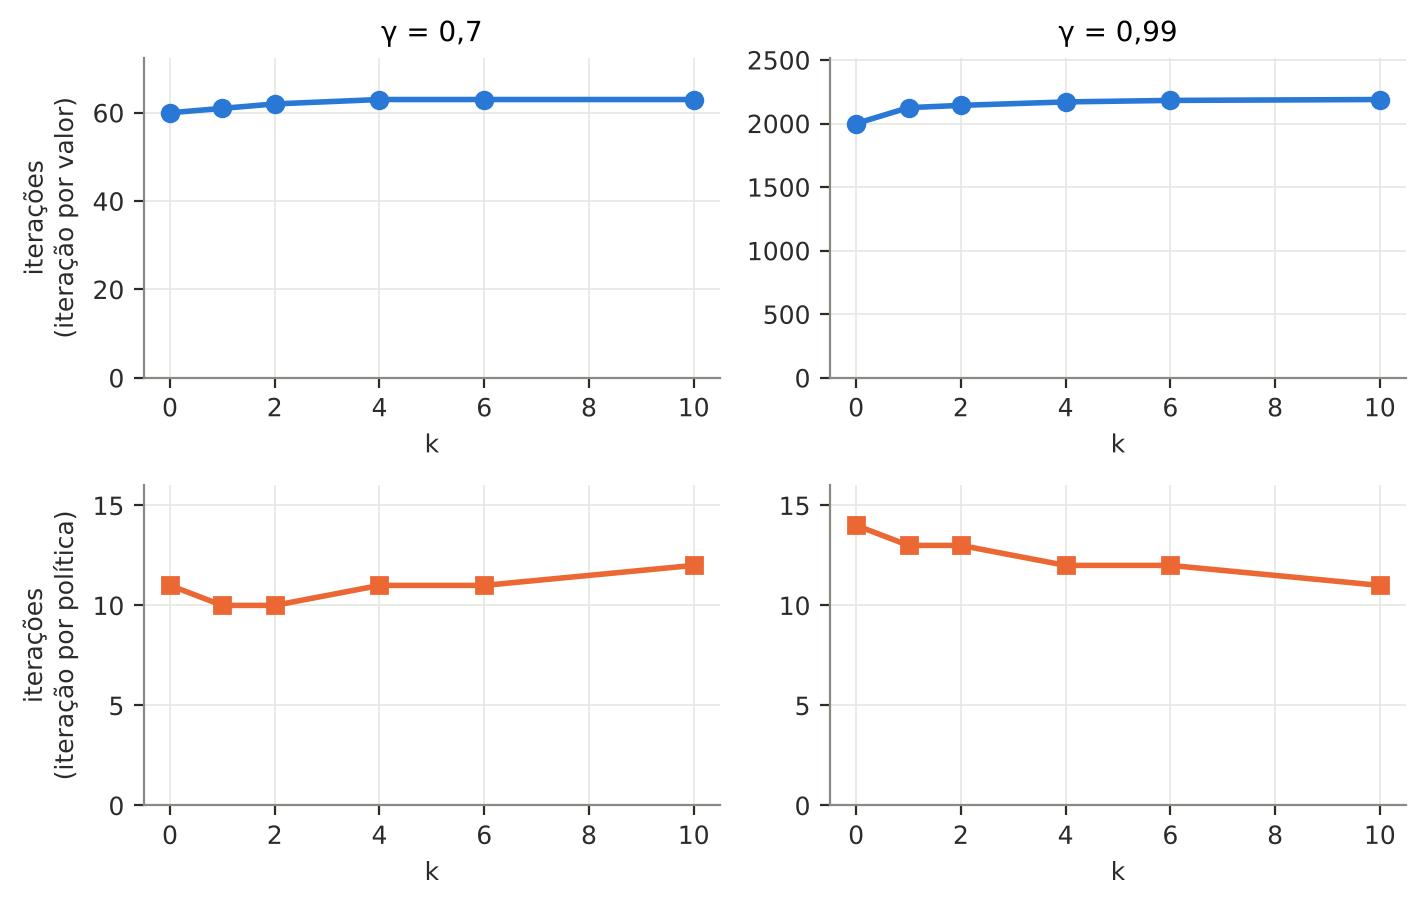
\includegraphics[width=0.8\textwidth]{fig/f5.png}
\caption{Número de iterações em função de $k$.}
\label{fig:iteracoes}
\end{figure}

\subsection*{2a. Tempo e iterações em função de $k$}

O número de iterações quase não muda com $k$. Foram cerca de 60 ($\gamma = 0{,}7$) e 2000 a 2200 ($\gamma = 0{,}99$) na iteração por valor, e de 10 a 14 na iteração por política. O que controla as iterações da iteração por valor é $\gamma$, porque o erro cai por um fator $\gamma$ a cada iteração, ou seja, a convergência é exponencialmente rápida.

O tempo cresce com $k$. Com $\gamma = 0{,}99$ a iteração por valor passou de 90~s para 270~s e a iteração por política de 95~s para 560~s. Cada iteração fica mais cara porque, com $k$ maior, a transição de captura leva a mais estados possíveis do cachorro e as matrizes ficam mais densas. A iteração por política faz poucas iterações, mas cada uma inclui uma avaliação completa, e por isso ela foi mais lenta que a iteração por valor, chegando a levar de duas a três vezes mais tempo nos valores altos de $k$.

\subsection*{2b. A política ótima muda com $k$?}

Comparar as ações diretamente não basta, porque a política ótima não é única. A mudança foi medida aplicando a política ótima de um valor $k'$ ao modelo de outro valor $k$, de duas formas, pela fração de estados em que sua ação não é ótima, e pelo valor perdido, obtido avaliando essa política no modelo $k$ e comparando com o valor ótimo (Figura~\ref{fig:mudanca}).

\begin{figure}[H]
\centering
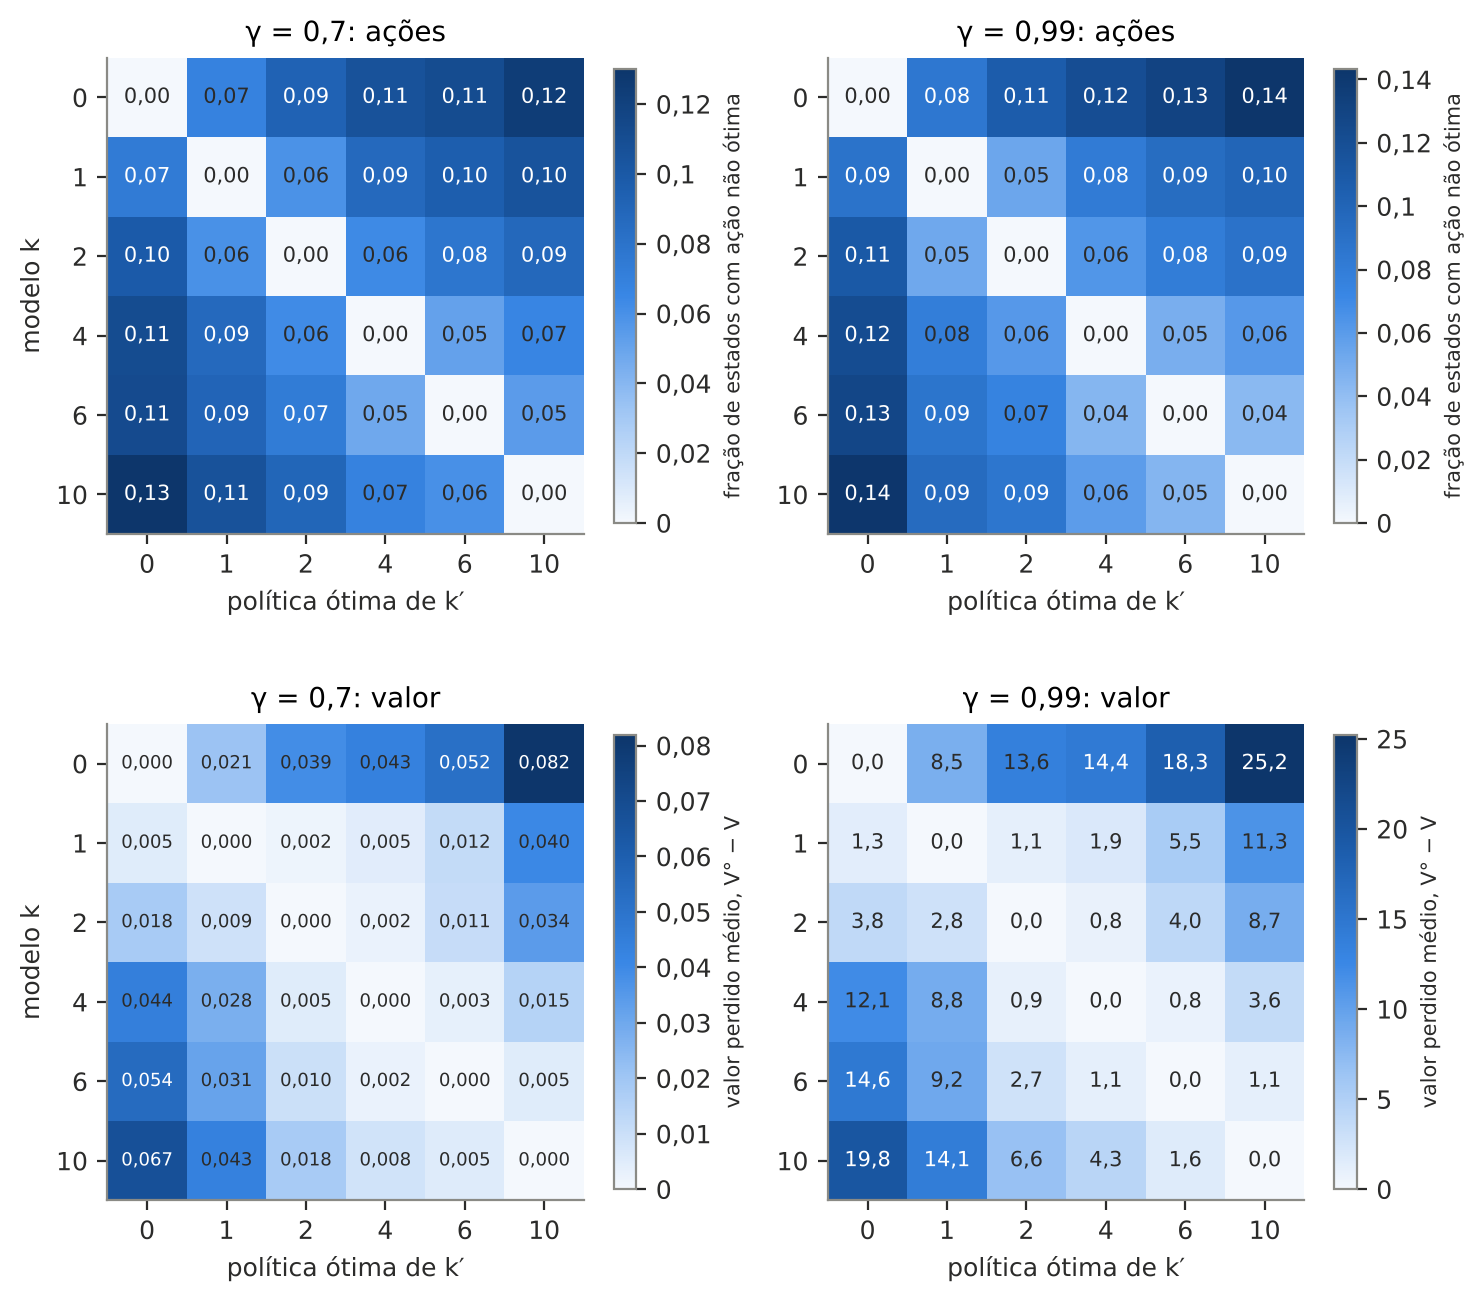
\includegraphics[width=0.85\textwidth]{fig/f7.png}
\caption{Política ótima de $k'$ (colunas) usada no modelo $k$ (linhas), com a fração de estados com ação não ótima (acima) e valor perdido médio (abaixo).}
\label{fig:mudanca}
\end{figure}

A política ótima muda com $k$, e mais quanto mais distantes os valores de $k$. Entre vizinhos, como 4 e 6, a ação muda em cerca de 5\% dos estados, enquanto entre 0 e 10 muda em cerca de 13\%. Com $\gamma = 0{,}7$ o valor perdido é pequeno. Com $\gamma = 0{,}99$ ele é grande nos extremos, pois usar a política de $k = 10$ no mundo $k = 0$ perde cerca de 25, o triplo do próprio valor ótimo desse caso. O caso $k = 0$, em que a captura não custa nada, é o mais diferente de todos. As duas medidas se complementam, porque frações parecidas de ações diferentes podem custar valores bem diferentes.

\subsection*{2c. Comparação com as políticas do item 1}

A ordem ótima, gulosa, aleatória vale em todos os cenários (Figura~\ref{fig:politicas}). Com $\gamma = 0{,}99$, a gulosa perde em média de 15 a 18 em relação à ótima, e cerca de 30 em $k = 0$, e escolhe uma ação não ótima em cerca de um quarto dos estados. Com $\gamma = 0{,}7$ as políticas ficam próximas, pelo motivo visto em 1b.

\begin{figure}[H]
\centering
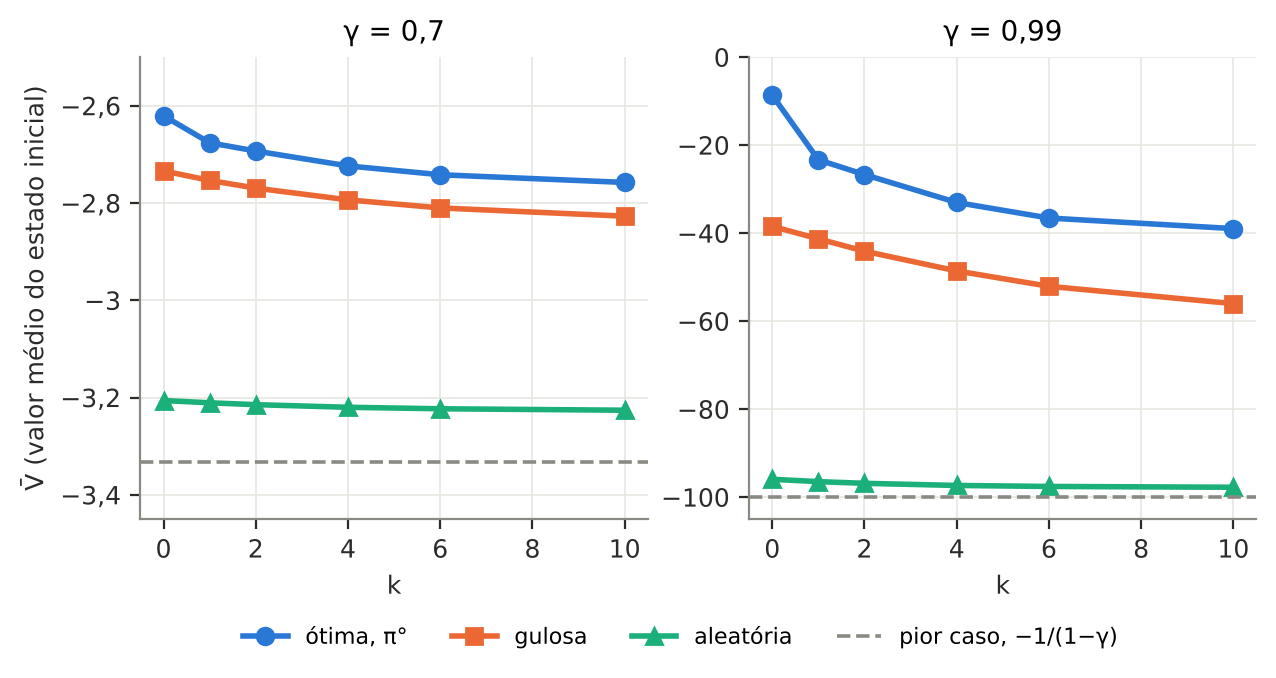
\includegraphics[width=0.85\textwidth]{fig/f6.png}
\caption{$\Vbar$ das políticas ótima, gulosa e aleatória em função de $k$.}
\label{fig:politicas}
\end{figure}

A maior diferença é em $k = 0$ com $\gamma = 0{,}99$, em que o valor da ótima é mais de quatro vezes melhor. Uma explicação provável, ainda não verificada, é que a ótima aproveita o tempo com a sala limpa para ficar perto do cachorro e limpar o próximo xixi rápido, enquanto a gulosa só se move depois que o xixi aparece.

% =====================================================================
\section{Item 3: Q-learning}

Foram escolhidos os cenários ($k = 4$, $\gamma = 0{,}7$), de horizonte curto, e ($k = 10$, $\gamma = 0{,}99$), o mais difícil, em que a gulosa ainda perde bastante para a ótima. Cada um foi treinado com três sementes e trajetórias de 1, 3 e 10 milhões de passos (Figura~\ref{fig:qlearning}). Como a mesma semente gera a mesma trajetória, as execuções mais curtas são o início das mais longas, e os três pontos equivalem a medir a qualidade da política em três momentos do mesmo treino.

\begin{figure}[H]
\centering
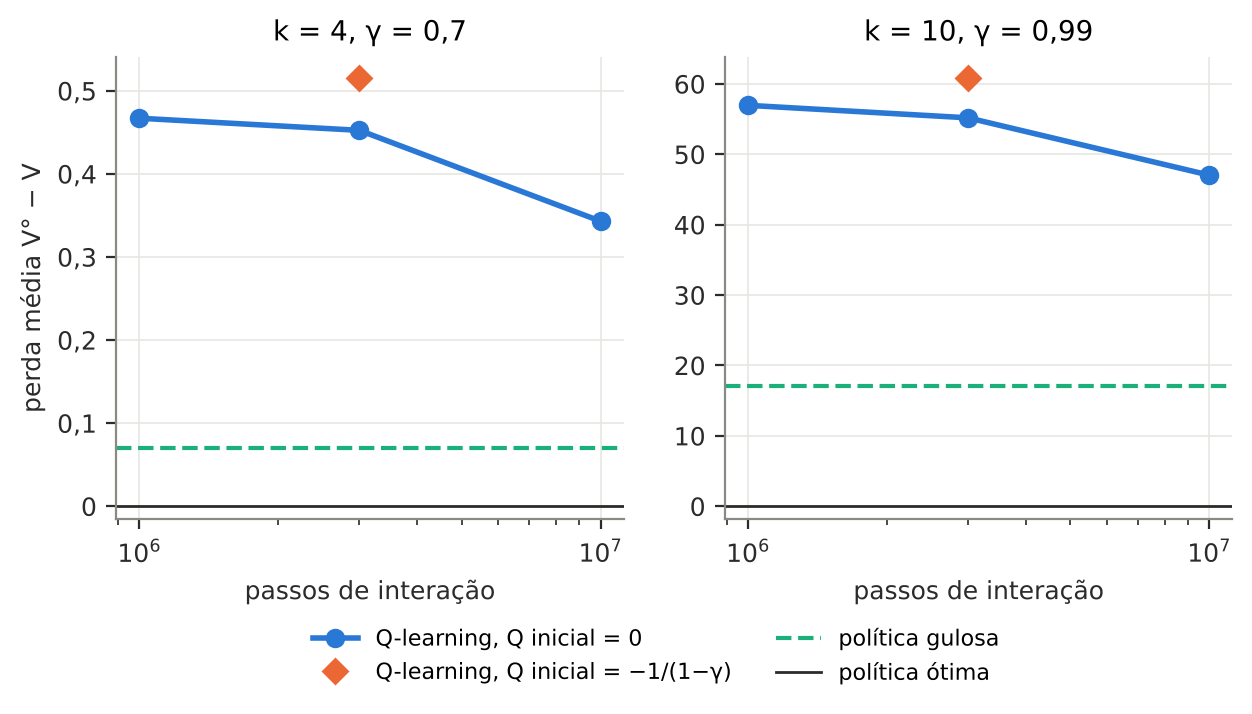
\includegraphics[width=0.85\textwidth]{fig/f8.png}
\caption{Perda média da política aprendida em função do número de passos (média de três sementes). O losango é a inicialização $Q = -1/(1-\gamma)$.}
\label{fig:qlearning}
\end{figure}

\subsection*{3a. Inicialização de $Q$ com recompensas não-positivas}

Como as recompensas são no máximo 0, todo valor de $Q$ é no máximo 0, e $Q = 0$ é o maior valor possível. Assim, cada ação experimentada recebe recompensas negativas e passa a parecer pior que as não experimentadas, o que leva o agente a explorar. Isso ajuda a cumprir a condição de que todo par $(s, a)$ seja visitado. Por outro lado, com $\gamma = 0{,}99$ os valores verdadeiros ficam entre cerca de $-40$ e $-100$, longe do palpite inicial, e com a taxa $\alpha_m = 1/m$ esse viés inicial é corrigido devagar, o que contribui para a convergência lenta vista em 3b.

A outra opção natural, que usa o valor de $\gamma$, é inicializar no menor valor possível, $-1/(1-\gamma)$, o retorno de uma sala suja para sempre. Nela, quando a sala está suja, o alvo da atualização é igual ao valor atual e $Q$ não muda, de modo que as ações ficam empatadas e o agente repete sempre a mesma. Com 3 milhões de passos ela visitou só cerca de 1\% dos pares $(s, a)$, contra mais de 85\% com $Q = 0$, e ficou pior até que a política aleatória. Portanto $Q$ deve começar em 0.

\subsection*{3b. Comparação com os métodos baseados em modelo}

Em qualidade, o Q-learning ficou bem atrás. Com 10 milhões de passos, a perda média foi de $0{,}34$ e 47, contra $0{,}07$ e 17 da gulosa e zero da iteração por valor e da iteração por política, ou seja, o resultado ficou entre a aleatória e a gulosa. A melhora com o número de passos é clara, mas lenta.

O motivo está nas condições de convergência do Q-learning, que exigem que cada par $(s, a)$ seja visitado muitas vezes. São cerca de 3 milhões de pares, e 10 milhões de passos dão só umas 3 visitas por par, pouco para estimar valores que dependem de centenas de passos futuros. Os métodos com modelo usam as probabilidades de transição exatas, e cada consulta ao modelo devolve a distribuição inteira do próximo estado, enquanto um passo de interação devolve uma única amostra.

Em tempo, 10 milhões de passos levaram cerca de 2 minutos nos dois cenários. A iteração por valor levou 4~s no cenário curto e 4,5 minutos no longo, mais a construção do modelo. Os métodos de iteração precisam do modelo, e a vantagem do Q-learning é dispensá-lo, mas neste exercício o modelo está disponível, e com ele a solução é melhor.

% =====================================================================
\section{Considerações finais}

A gulosa é muito melhor que a aleatória, mas ainda está longe da ótima com $\gamma = 0{,}99$. O custo de captura $k$ piora todas as políticas e muda a política ótima. A avaliação iterativa e a iteração por valor foram as opções mais eficientes, e o tempo de todos os métodos cresce com $k$ pela densidade das matrizes, não pelo número de iterações. O Q-learning, com poucas visitas por par estado-ação, não alcançou a gulosa, e a inicialização $Q = 0$ se mostrou essencial para explorar.

\end{document}
